\vspace{-0.5cm}
\section{\label{sec:ir}The \framework{} IR}
The main goal of \framework{}'s multi-layer intermediate representation is to simplify the implementation of scheduling commands by applying them in a specific order.
This section illustrates why, and describes the layers of the \framework{} IR.
\vspace{-0.4cm}
\subsection{Why a Multi-layer IR ?}

Most intermediate representations use memory to communicate between program statements.  This creates memory-based dependencies in the program, and forces data-layout to be chosen before deciding how the code is optimized and mapped to hardware.  Optimizing a program for different hardware architectures usually requires modifying the data-layout and eliminating memory-based dependencies since they restrict optimization~\cite{maydan1992data}.  Thus, any data-layout specified before scheduling must be undone to allow more freedom for scheduling, and the code must be adapted to use the data-layout best-suited for the target hardware.
Applying these data-layout transformations and the elimination of memory-based dependencies is challenging~\cite{gupta1997privatization,autoPrivatPeng,li_array_1992,feautrier_array_1988,midkiff_automatic_2012,maydan_array-data_1993,lefebvre_automatic_1998,Qui00,Darte_contraction_2005}.

Another example that makes code generation complicated is mapping buffers to shared and local memory on GPU.  The amount of data that needs to be copied to shared memory and when to perform synchronization all depend on how the code is optimized (for example,  whether the code has two-level tiling or not).  The same applies to deciding the amount of data to send or receive when generating distributed code.   Therefore, communication management, buffer mapping to memory hierarchies, and synchronization should not be done before scheduling.

\framework{} addresses these challenges by using a multi-layer IR that fully separates the architecture-independent algorithm from loop transformations, data-layout and communication.
The top layer representation describes the pure algorithm using producer-consumer relationships without memory locations.
The second layer specifies the order of the computations, along with which processor computes each value; this layer is suitable for performing a vast number of optimizations without dealing with concrete memory layouts.
The third layer specifies where to store intermediate data before they are consumed.  The fourth layer adds all the necessary communication and synchronization operations.
%The multi-layer design makes the algorithm portable and makes it easier to perform each program transformation at the right layer of abstraction.
%The multi-layer design simplifies the implementation of code transformations in the compiler.  Each program transformation is performed at the right layer of abstraction.

The separation of layers defines a specific order in which optimizations are applied and ensures that compiler passes in a given layer need not worry about modifying or undoing a decision made in an earlier layer.  For example, the phase that specifies the order of computations and where they occur can safely assume that no data-layout transformations are required, greatly simplifying the phase.
This simple assumption allows \framework{} to avoid the need to rely on a large body of research that focuses on data-layout transformations to allow scheduling~\cite{gupta1997privatization,autoPrivatPeng,li_array_1992,feautrier_array_1988,midkiff_automatic_2012,maydan_array-data_1993,lefebvre_automatic_1998,Qui00,Darte_contraction_2005}.

\subsection{Background}

In this section, we provide an overview of two main concepts used in the polyhedral model: \emph{integer sets} and \emph{maps}. These two concepts will be used in later sections to define the different IR layers.

\emph{Integer sets} are used to represent the iteration domain of code while \emph{maps} are used to represent the memory accesses and to transform iteration domains and memory accesses (apply loop nest and memory access transformations).  More details and formal definitions for these concepts are provided in~\cite{verdoolaege_isl:_2010,pencil_pact,polyhedral}.

An \emph{integer set} is a set of integer tuples described using affine constraints.  An example of a set of integer tuples is \polyc{$\{(1,1); (2,1); (3,1); (1,2); (2,2); (3,2)\}$}
Instead of listing all tuples in a set, we describe the set using affine constraints over loop iterators and symbolic constants: \polyc{$\{S(i,j): 1 \leq i \leq 3 \wedge 1 \leq j \leq 2\}$} where $i$ and $j$ are the dimensions of tuples in the set.

A \emph{map} is a relation between two integer sets.  For example
\polyc{$\{S1(i,j) \rightarrow S2(i+2,j+2) : 1 \leq i \leq 3 \wedge 1 \leq j \leq 2\}$}
is a map between tuples in the set S1 and tuples in the set S2 (e.g. the tuple \poly{$S1(i,j)$} maps to the tuple \poly{$S2(i+2,j+2)$}).

All sets and maps in \framework are implemented using the Integer Set Library (ISL)~\cite{verdoolaege_isl:_2010}. We also use the ISL library notation for sets and maps throughout the paper.

%Polyhedral sets and relations are described using affine (linear) constraints over loop iterators and program parameters (invariants) and are implemented in \framework using ISL~\cite{verdoolaege_isl:_2010}.  We use a combination of classical extensions to the polyhedral model in order to support non-affine iteration spaces; these extensions are sufficient for large classes of programs in practice~\cite{benabderrahmane_polyhedral_2010,pencil}, and in particular to our areas of interest: dense linear algebra and tensor algebra, stencils, image processing and deep neural networks.

\subsection{The Multi-Layer IR}

\begin{figure}
 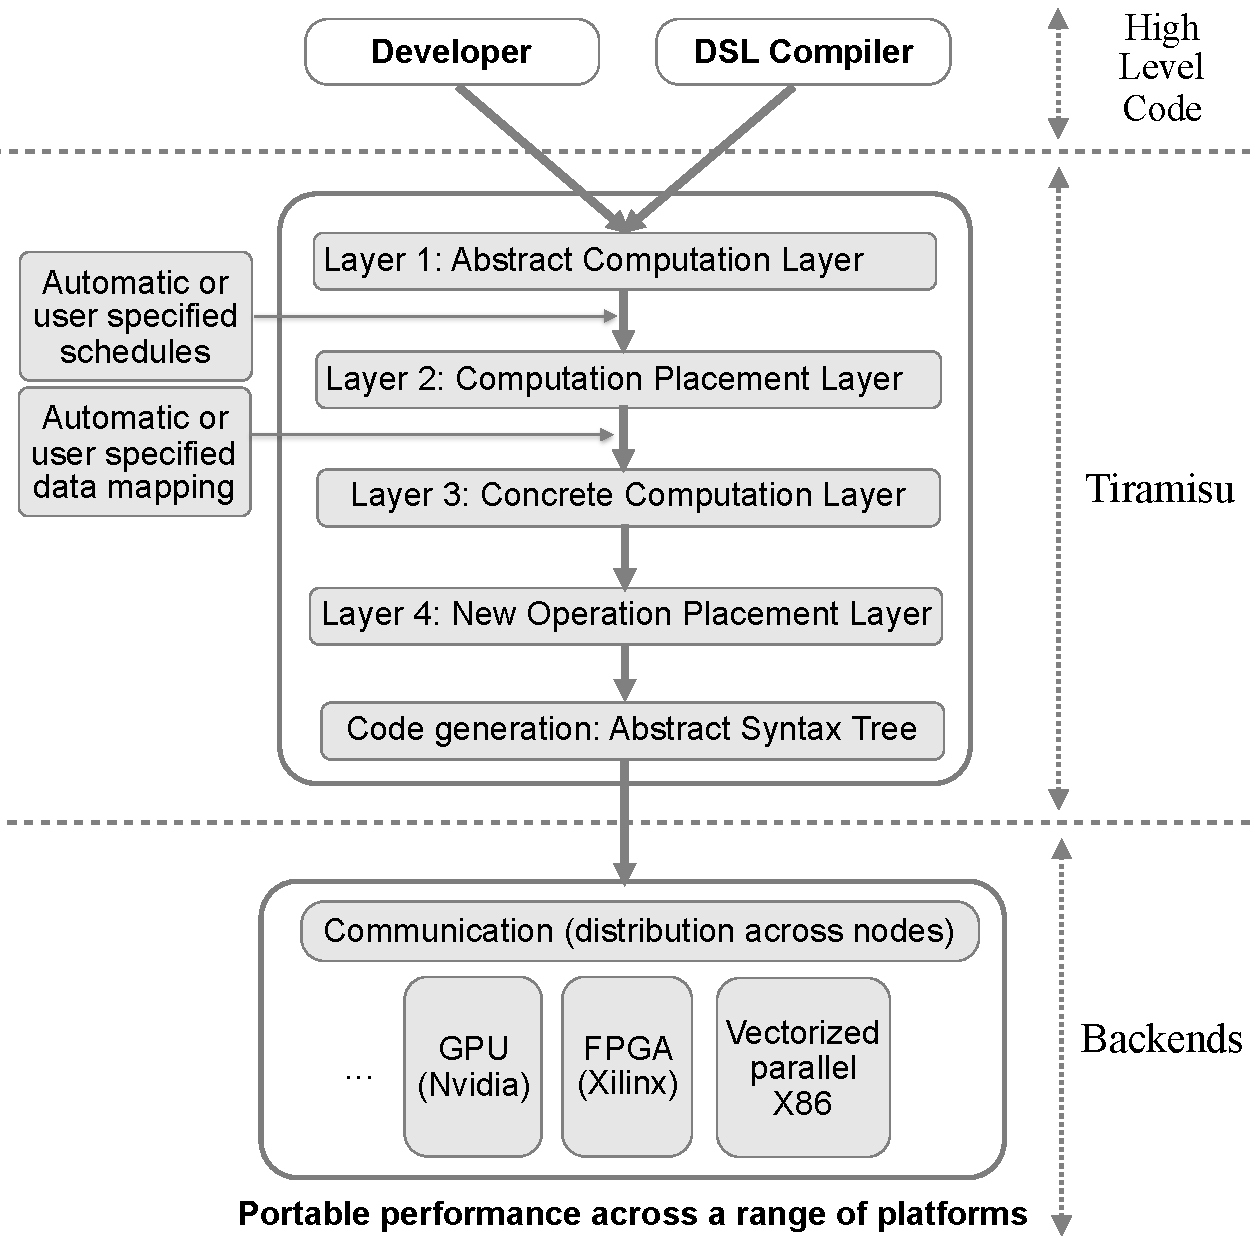
\includegraphics[scale=0.28]{./figures/fista.pdf}
 \vspace{-0.25cm}
 \caption{\framework overview}
 \label{fig:overview}
 \vspace{-0.5cm}
\end{figure}

A typical workflow of using \framework is illustrated in Figure~\ref{fig:overview}.  The user writes the first layer of \framework{} (which is the pure algorithm) and then provides a set of scheduling commands.  The first layer of the IR is then transformed to lower layers, and finally \framework{} generates LLVM IR or other appropriate low-level IR.
\framework{} uses \emph{integer sets} to represent each of the four IR layers and uses \emph{maps} to represent transformations on the iteration domain and data-layout.
The remainder of this section describes the four layers of the \framework IR.

\vspace{-0.25cm}
\subsubsection{Layer I (\Layerone)}
\label{layer1}

Layer I of \framework{} specifies the algorithm without specifying the schedule (when and where the computations occur) or how data should be stored in memory (data-layout) or communication. As this level has no notion of data location, values are communicated via explicit producer-consumer relationships.

Let us take the example of the code in Figure~\ref{fig:algorithm} and let us only consider the computation \texttt{by} for simplicity. It is represented in Layer I as follows.

\begin{lstlisting}[language=C,escapechar=@]
@\poly{$\{by(i, j, c): 0\leq i<N-2 \wedge 0\leq j<M-2 \wedge 0\leq c<3\}$}@:(bx(i,j,c)+bx(i+1,j,c)+bx(i+2,j,c))/3
\end{lstlisting}

The first part of this line, which is
\poly{$\{by(i,j,c): 0\leq i<N-2 \wedge 0\leq j<M-2 \wedge 0\leq c<3\}$}, specifies the iteration domain of the statement, while the second part, $(bx(i,j,c)+bx(i+1,j,c)+bx(i+2,j,c))/3$, is the computed expression.
The iteration domain is the set of tuples \poly{$by(i,j,c)$} such that \poly{$0\leq i< N-2 \wedge 0\leq j< M-2 \wedge 0\leq c < 3$}.
Computations in Layer I are not ordered;  declaration order does not affect the order of execution, which is specified in Layer II. 

\subsubsection{Layer II (\Layertwo)}
\label{layer2}

Layer II of \framework{} specifies the order of execution of computations and the processor on which they execute.  This layer does not specify how intermediate values are stored in memory; this simplifies optimization passes since these transformations do not need to perform complicated data-layout transformations.  The transformation of Layer I into Layer II is done automatically using scheduling commands.

Figure~\ref{fig:mainexample}-\codetwo{} (right) shows the first optimized version of the code, produced by the set of scheduling and data-layout commands on the left side.
The corresponding Layer II representation for the \texttt{by} computation is shown below

\noindent
\poly{$\{ by(1, i0 (gpuB), j0 (gpuB), i1 (gpuT), j1 (gpuT), c): i0=floor(i, 32) \wedge j0=floor(j, 32) \wedge i1=i\%32 \wedge j1=j\%32 \wedge 0\leq i<N-2 \wedge 0\leq j<M-2 \wedge 0\leq c<3\}$} : (bx(i,j,c)+bx(i+1,j,c)+bx(i+2,j,c))/3

Computations in Layer II are ordered based on their lexicographical order\footnote{For example the computation $S0(0, 0, 0)$ is lexicographically before the computation \mbox{$S0(0, 0, 1)$} and the computations $S0(0, i, 0)$ are lexicographically before the computations $S0(1, i, 0)$}.  The set (purple text in the previous example), is an ordered set of computations.
The tag \emph{gpuB} for the dimension $i0$ and $j0$ indicates that each iteration ($i0,j0$) is mapped to the GPU block ($i0,j0)$. In Layer II, the total ordering of these tuples determines the execution order.

Unlike the first layer, computations in this layer are ordered and assigned to a particular processor (we know when and where they will run).  This order is dictated by \textit{time dimensions} and \textit{\processor dimensions}.  Time dimensions specify the order of execution relative to other computations while \processor{} dimensions specify on which processor each computation executes.
The ordering of the time dimensions determines the execution order of each computation.
\Processor{} dimensions only indicate where computations run, and
are distinguished from time dimensions using tags, which consist of a processor type followed by
zero or more properties.  Currently, \framework{} supports the following space tags:

{
\centering
{
    \footnotesize
    \setlength\tabcolsep{5pt}
    \begin{tabular}{ll}
        %\hline
        \texttt{cpu} & the dimension runs on a CPU in a shared memory system \\
        %\hline
        \texttt{node} & the dimension maps to nodes in a distributed system \\
        \texttt{gpuT} & the dimension maps to a gpu thread dimension. \\
        \texttt{gpuB} & the dimension maps to a gpu block dimension.\\
    \end{tabular}
}
}

Tagging a dimension with a processor type indicates that the dimension should be distributed over processors of that type; for example, tagging a dimension with \emph{cpu} will execute each iteration of that loop dimension on a separate CPU.

Other tags that \framework{} supports and that describe how a dimension should be optimized include:

{
\centering
{
    \footnotesize
    \setlength\tabcolsep{5pt}
    \begin{tabular}{ll}
        %\hline
        \texttt{vec(s)} & vectorize the dimension (\emph{s} is the vector length)\\
        %\hline
        \texttt{unroll} & unroll the dimension\\
        %\hline
    \end{tabular}
}
}

Computations mapped to the same processor are ordered by projecting the computation set onto the time dimensions and comparing their lexicographical order.

\subsubsection{Layer III (\Layerthree)}
\label{layer3}

Layer III makes the data-layout concrete by specifying where intermediate values are stored.  Any necessary buffer allocations/deallocations are also constructed in this level.  This layer is generated automatically from Layer II by applying the scheduling commands for data mapping.

The \layerthree layer specifies memory locations for storing computed values.  It consists of the Layer II representation along with allocation/deallocation statements, and a set of \emph{access relations},
which map a computation from Layer II to array elements read or written by that computation.  Scalars are treated as single-element arrays.  %Buffers used for storage are declared and allocated in this layer. 
For each buffer, an allocation statement is created, specifying the type of the buffer (or scalar) and its size.  Similarly, a deallocation statement is also added.

Possible data mappings in \framework include mapping computations to structures-of-arrays, arrays-of-structures, and contraction of multidimensional arrays into arrays with fewer dimensions or into scalars.  It is also possible to specify more complicated accesses such as the storage of computations $c(i,j)$ into the array elements $c(i\%2,j\%2)$ or into $c(j,i)$.

Layer III adds data-layout mapping to Layer II, concretizing where each computation is stored (declarations of memory buffers and scalars are also introduced in this layer, based on the schedule).

In the example, setting the data access using\\ \texttt{by.store\_in({c,i,j})}\\
indicates that the result of the computation \poly{$by(i, j, c)$} is stored in the array element \poly{$by[c,i,j]$}. This command generates the following map in layer III:

\noindent
\poly{$\{by(1, i0 (gpuB), j0 (gpuB), i1 (gpuT), j1 (gpuT), c)\rightarrow by[c,i0*32+i1,j0*32+j1]: i0=floor(i, 32) \wedge j0=floor(j, 32) \wedge i1=i\%32 \wedge j1=j\%32 \wedge 0\leq i<N-2 \wedge 0\leq j<M-2 \wedge 0\leq c<3\}$}

Data mapping in \framework is an affine relation that maps a computation from Layer II to a buffer element; scalars are single-element buffers.  \framework allows any data-layout mapping that can be expressed as an affine relation.

\subsubsection{Layer IV (\Layerfour)}
\label{layer4}

Layer IV adds synchronization and communication operations to the representation,  as well as scheduling when statements for buffer allocation/deallocation occur.  This layer is generated automatically from Layer III by applying user-specified commands.

In this layer, communication statements (including synchronization) are added and scheduled (i.e., mapped to the time-\processor domain).
Any allocation or deallocation operation that was added in Layer III is also scheduled in this layer.
